\chapter{Experiment}
\label{chp:experiment}

To test the usability of the \ptakopet{} tool proposed in this thesis, we designed an experiment. This experiment aimed to classify and describe strategies users take when tasked to do outbound translation, as well as the final quality of the produced texts. It was the main focus of one of the papers connected to this thesis \citep{zouhar:ptakopet}.

\section{Setup}

The experiment was carried out remotely, in two phases. In the first phase, annotators were presented with a sequence of web pages and asked to produce a German sentence given a stimulus at each of them. In the second phase (\cref{sec:experiment_validation}), a highly-skilled speaker of German validated the outputs of the first phase.

QE highlighting in \ptakopet{} was enabled only for the first section, because the QE model did not perform well on out-of-domain sentences.

\subsection{Annotators}

There were 8 annotators in total, divided into two groups. The first one was composed of 4 people without advanced knowledge of English\footnote{Note that the annotators never needed to produce any English text in the experiment. Only one subset of the test data needed English comprehension.} and the second one consisted of 4 people with English level of at least C1 on the CEFR scale. All of the annotators had German knowledge of at most A1. We refer to these groups as bilingual and monolingual, respectively. The annotators' knowledge of German and English is summarized in \autoref{tab:annotator_languages}. Annotators with an English level equal to or below B2 were opted out of stimuli from the original SQuAD 2.0.

\begin{table}[H]
    \centering
    \begin{tabular}{| c c c |}
        \hline
        Annotator& English & German \\
        \hline
        C1& B2    & A0 \\
        C2& C1-C2 & A0 \\
        C3& B2    & A0 \\
        C4& B2    & A0 \\
        C5& B1-B2 & A0-A1 \\
        C6& C2    & A0-A1 \\
        C7& C1    & A0 \\
        \hline
    \end{tabular}
    \caption{\label{tab:annotator_languages} Language proficiency of English and German on the CEFR scale}
\end{table}

\subsection{Data}

For our experiment, we gathered input data and prompted users to reformulate a specific question or work with the text in some way. Each data section was meant to correspond to some real-life situations.
\subsubsection{Seeking help in technical issues}

For the best match with the QE training data (\cref{subsec:cs_de_wmt}), we extracted 35 stimuli (in Czech) from WMT 2017 English-German quality estimation dataset. The sentences describe technical issues when using common office or desktop publishing programs.

The annotators were expected to translate the description of the issue to German relying on machine translation and quality estimation tools.
% We expected the quality estimation tools to perform better given the overlap in the data (note that there was no overlap with the MT training data).
Furthermore, we think that explaining technical issues to IT support in an unknown language is a common outbound translation use case. An example of a technical issue is in \cref{fig:tech_example} (translated to English).

\begin{figure}[ht]
    \noindent\rule{\linewidth}{0.5pt}
    \textbf{Issue description:}
    
    The date format cannot be changed from Month-Day-Year to Day-Month-Year.
    
    \vspace{-0.2cm}\noindent\rule{\linewidth}{0.5pt}\vspace{-0.3cm}
    \caption{\label{fig:tech_example} Example description of a technical issue
    from the experiment dataset.}
\end{figure}

\subsubsection{Common administrative issues}

The next 30 test stimuli in the experiments provided a source text in Czech with a piece of factual information (a short span in the text) highlighted. The annotators were supposed to formulate questions that ask for this factual information.

This data was collected from the instructions on how to proceed in various administrative topics at the Municipal District of Prague 6.\footnotehref{https://www.praha6.cz/codelat/index.php}{praha6.cz/codelat/index.php} This use case is inspired by the day to day problems of citizens living in a foreign city. With the help of MT, they can get the gist of regulation or relevant document but they may need to ask the administration for some clarification or a specific detail.

%relevant not only for gisting but also for outbound
%translations:
%foreigners living in a city may need to ask questions relevant to the original
%text with administrative
%information.

An example of an administrative issue stimulus can be seen in \cref{fig:admin_example}. For presentation purposes, we again translate the stimulus into English but the annotators saw Czech text and were expected to formulate the question in Czech so that MT produces a good German version.

\begin{figure}[ht]
    \noindent\rule{\linewidth}{0.5pt}
    \textbf{Paragraph with highlighted span:}
    
    Applicant pays {\underline{100 CZK}} when changing a surname that is derogatory, eccentric, ridiculous, garbled, or foreign.
    
    \vspace{-0.2cm}\noindent\rule{\linewidth}{0.5pt}\vspace{-0.2cm}
    \caption{\label{fig:admin_example} Example administrative topic and the
    factual information to ask for (the price) highlighted}
\end{figure}

\subsubsection{Encyclopedic knowledge: SQuAD 2.0}

The last section of the experimental data was based on the Stanford Question Answering Dataset 2.0 \cite{SQUAD-2.0} and its (machine-translated) Czech version.\footnote{Translation provided by Matúš Žilinec; the dataset is available at \href{https://zilinec.me/dl/datasets/squad/train-cs-v2.1.json}{zilinec.me/dl/datasets/squad/train-cs-v2.1.json}} The basic unit of SQuAD are paragraphs with spans. In the context of SQuAD 2.0, this means that there already existed a question for this span. In our experiment, we disregard the existing questions and ask our annotators to ask for the highlighted information again. We are thus creating additional questions for the SQuAD dataset, now in Czech.

An example of a paragraph from SQuAD 2.0 and questions we collected from the \ptakopet{} pilot study (again translated to English) can be seen in \cref{fig:squad_par}.

\begin{figure}[ht]
    \noindent\rule{\linewidth}{0.5pt}
    \textbf{Paragraph with highlighted span:}
    
     All of Chopin's compositions include {\underline{the piano}}. Most are for solo piano, though he also wrote two piano concertos, a few chamber pieces, and some songs to Polish lyrics. 
    
    \textbf{Sample questions asked by our annotators:}
    
    What do all Chopin's songs include?
    
    What musical instrument will we hear in virtually all Chopin's compositions?
    
    \vspace{-0.2cm}\noindent\rule{\linewidth}{0.5pt}\vspace{-0.3cm}
    \caption{\label{fig:squad_par} Paragraph from SQuAD with two questions for
    the underlined span}
\end{figure}

We were mostly interested in spans of text which had more questions in SQuAD already because such spans seemed easier to create questions for. The distribution of questions per span in SQuAD can be seen in \cref{tab:squad_distribution}: the vast majority of spans have only one question and having more than four questions per span is very rare.
%It suggests, that there exist lots of spans, which correspond to only one
%question, and gradually fewer spans with higher question rate.
The rightmost column shows how many of such spans were included in our experimental data.

\begin{table}[ht]
    \centering
    \begin{tabular}{| c c c |}
        \hline
        Questions & Number of spans & Occurences in \\
        per span & in SQuAD 2.0 & experiment data \\
        \hline
        1&   81619& 15\\
        2&    2303& 15\\
        3&     166& 15\\
        4&      13& 10\\
        5&       8&  5\\
        6&       1&  0\\
        \hline
        Total: & 84110  & 60 \\
        \hline
    \end{tabular}
    \caption{\label{tab:squad_distribution}SQuAD 2.0 span distribution}
\end{table}

In total, 60 paragraphs were chosen from SQuAD 2.0 randomly but respecting the intended distribution in the third column in \cref{tab:squad_distribution}. These paragraphs were machine-translated to Czech and the spans were transferred to Czech manually. Bilingual users then had half of the SQuAD paragraphs in Czech and half in English, monolingual users saw only the Czech paragraphs. No user saw the same paragraph in both English and Czech.

\subsubsection{Annotation task composition}

The overall composition of types of stimuli is shown in \cref{tab:stimuli_composition}. The bilingual group received half of the SQuAD stimuli in Czech and half in English. The monolingual group received all the SQuAD stimuli in Czech.

\begin{table}[H]
    \centering
        \begin{tabular}{| l | c c |}
            \hline 
            Stimuli & monolingual & bilingual \\
            \hline
            Technical issues & 35 & 35 \\
            Administrative issues & 30 & 30 \\
            SQuAD 2.0 & 0 & 30 \\
            SQuAD 2.0 Czech & 60 & 30 \\
            \hline
            Total & 125 & 125 \\
            \hline
        \end{tabular}
    \caption{\label{tab:stimuli_composition} Overall composition of the input stimuli}
\end{table}

All of the annotators overlap fully in technical and administrative issues. The monolingual annotators overlap entirely within the group and 50\% with the bilingual group. Such overlaps are necessary for studying the same stimulus answers variations.

\subsection{User Interface}

The \ptakopet{} frontend version used for the experiment is stored in the git repository under \texttt{v-pilot} tag. It was later improved and the most up to date public version is described thoroughly in \cref{chp:usage}. The user interface is different for experiments than for public use. The experiment user interface can be seen in \autoref{fig:experiment/stimuli_ui.png}. Apart from the standard three text boxes, the settings section is hidden and at the top, there is a stimulus briefly describing the task, as well as the text in question.

\figcap{experiment/stimuli_ui.png}{Screenshot of \ptakopet{} for annotators with a stimulus from the translated version of SQuAD 2.0}

\subsection{Technical details} \label{subsec:experiment:technical_details}

All the relevant experiment files and scripts together with their usage are discussed in detail in \cref{sec:dev_doc:experiment}. 

\subsubsection{Data gathering}

Throughout the \ptakopet{} annotation, we logged various data, while the users interacted with \ptakopet{}. The list of each logged information is shown in \autoref{tab:annotation_info_1} and the description of each information type is in \autoref{tab:annotation_info_2}. Additionally, each logged action contained Unix timestamp. The logs are stored for in files with \texttt{<userID>.log} scheme.

The logged data for each user is stored in CSV format in one file, thus interleaving multiple tables. Each row is prefixed with an extra column, describing the logged action. Thus the file can be easily grepped to extract correctly formatted tables.

\begin{table}[H]
    \centering
    \begin{tabular}{| l | l l |}
        \hline
        Action code & Logged information & Description \\
        \hline
        START      & - & The user logs in \\
        NEXT       & SID & A stimuli is shown \\
        CONFIRM    & SID, TEXT1, TEXT2 & User accepts solution \\
        SKIP       & SID, REASON & User skips stimuli \\
        TRANSLATE1 & SID, TEXT1, TEXT2 & Forward translation is displayed \\
        TRANSLATE2 & SID, TEXT2, TEXT3 & Backward translation is displayed \\
        ESTIMATE   & SID, ESTIMATION & Quality estimation is highlighted \\
        ALIGN      & SID, ALIGNMENT  & Source complexity is highlighted \\
        \hline
        PARAPHRASE & PARAPHRASES & Paraphrases are displayed \\
        NOTE       & SID, MESSAGE  & User typed in a note \\
        \hline
    \end{tabular}
    \caption{\label{tab:annotation_info_1} Logged information from \ptakopet{} users for each of their actions. Last two logging actions were not used for the pilot experiment.}
    
    \bigskip 
    \begin{tabular}{| l l |}
        \hline
        Logged information & Description \\
        \hline
        SID & Identifier of the relevant stimuli  \\
        TEXT1 & Content of the source text area \\
        TEXT2 & Content of the target text area \\
        TEXT3 & Content of the backward translation text area \\
        ESTIMATION & Quality estimation data \\
        ALIGNMENT & Source to target word alignment \\
        REASON & User's motive for skipping answering the stimuli \\
        \hline
    \end{tabular}
    \caption{\label{tab:annotation_info_2} Description of logged information from \ptakopet{} users}
\end{table}

\subsubsection{Baked queue stimuli preparation}

We want the stimuli to be distributed randomly but in a fixed manner. We also want to know the distribution of stimuli to users beforehand so that we can regenerate it in case of any anomalies. For this, we use the concept of \textit{baked queues}. For every user, we generate a fixed array of stimuli that will be shown to them.

The pool size of stimuli per domain is hardcoded as Technical issues: 35, Administrative issues: 30, SQuAD Czech: 60, SQuAD: 60.

\section{Results} \label{sec:experiment_validation}

The results of this experiment were published in \cite{zouhar:ptakopet} and this section uses whole paragraphs and tables from this paper.

\subsection{Basic statistics}

We refer to sequences of log entries related to the same stimulus as segments. The number of finished segments, as well as their average duration in every domain, is shown in \cref{tab:segments_avg_duration}. Since the differences in duration between each segment were not high (min 90s, max 106s), we concluded that the users employed similar strategies across all domains and that no domain was exceptionally difficult nor easier than the others.

\begin{table}[ht]
    \centering
    \begin{tabular}{| l c c |}
        \hline
        Domain & Segments & Average duration \\
        \hline
        SQuAD 2.0 & 141 & 100s  \\
        SQuAD 2.0 Czech & 346 & \ 94s \\
        Technical issues & 268 & 107s \\
        Administrative issues & 246 & \ 90s \\
        \hline
        All & 1001 & \ 98s \\
        \hline
    \end{tabular}
    \caption{\label{tab:segments_avg_duration} Number of segments and average duration across all users per domain in collected data}
    \vspace{-0.9cm}
\end{table}

\subsection{Types of edits}

Some of the stimuli were skipped, mostly because the annotators did not have enough confidence in the MT system's performance (for a given stimulus) and were unable to produce a better result. We describe such segments as \textit{skipped} as opposed to \textit{finished}. From the finished ones, about a quarter of the segments were written linearly (no edits or deletions in already written text). Such segments are denoted as \textit{linear} as opposed to segments, which had some edits in already written parts (\textit{with edits}). The number of skipped, finished, linear and edited segments can be seen in \cref{tab:dr1}.

We see that the proportion of skipped segments (i.e., segments where the annotator failed to produce an output they could accept) is not excessively high. The easiest to process were administrative issues (5.7\,\% skipped segments) and the hardest was the technical issues (10.8\,\%). SQuAD reached 7.8\,\% (English) and 7.5\,\% (Czech) of skipped segments.

Of the finished segments, most (72\%) were edited and not just linearly written (28\%). Additionally, in technical issues, the stimulus was the description of the technical problem itself, so the annotators could choose to simply copy this text and paste it in the input window. The number of occurrences of this behavior is described in the table as \textit{init copy} (60\% of all edited). We also measured the number of final inputs, which matched the initial stimulus (\textit{Copy \& submit}, 6\% of all edited).

\newcommand{\tbofall}{\multirow{2}{*}{\small (of all)}}
\newcommand{\tboffin}{\multirow{2}{*}{\small (of fin.)}}
\newcommand{\tbofedt}{\multirow{2}{*}{\small (of edt.)}}
\newcommand{\tbperc}[1]{\small (#1\%)}

\begin{table}[ht]
    \centering
    \begin{tabular}{| c l r r|}
        \hline
        Domain & Description & Segments & Ratio \\
    \hline
        \multirow{4}{*}{SQuAD 2.0} & Skipped & 11 \tbperc{8} & \tbofall{} \\
         & Finished & 130 \tbperc{92} & \\
         \cline{2-4}
         & Linear & 52 \tbperc{40} & \tboffin{} \\
         & With edits & 78 \tbperc{60} & \\
    \hline
        \multirow{4}{*}{\parbox{30mm}{\centering SQuAD 2.0 Czech}} & Skipped & 26 \tbperc{8} & \tbofall{} \\
         & Finished & 320 \tbperc{92} &\\
         \cline{2-4}
         & Linear & 110 \tbperc{34} & \tboffin{} \\
         & With edits & 210 \tbperc{66} & \\
    \hline
        \multirow{4}{*}{\parbox{30mm}{\centering Tech issues}} & Skipped & 29 \tbperc{11} & \tbofall{} \\
         & Finished & 239 \tbperc{89} & \\
         \cline{2-4}
         & Linear & 27 \tbperc{11} & \tboffin{} \\
         & With edits & 212 \tbperc{89} & \\
          \cline{2-4}
         & Init copy & 127 \tbperc{60} & \tbofedt{} \\
         & Copy \& submit \hspace{-0.3cm} & 13 \tbperc{6} & \\
    \hline
        \multirow{4}{*}{\parbox{30mm}{\centering Administrative issues}} & Skipped & 14 \tbperc{6} & \tbofall{} \\
         & Finished & 232 \tbperc{94} & \\
         \cline{2-4}
         & Linear & 70 \tbperc{30} & \tboffin{} \\
         & With edits & 162 \tbperc{70} & \\
    \hline
        \multirow{4}{*}{All} & Skipped & 80 \tbperc{8} & \tbofall{} \\
         & Finished & 921 \tbperc{92} & \\
         \cline{2-4}
         & Linear & 259 \tbperc{28} & \tboffin{} \\
         & With edits & 662 \tbperc{72} & \\
    \hline
    \end{tabular}
    \caption{\label{tab:dr1} Number of skipped, finished, linear and edited segments per domain in collected data together with percentage of all, finished or edited segments.}
\end{table}

We then focused on the segments, which were further edited. We tried to extract the first input the annotator expected to be successful. We call this input \textit{first viable} and choose it heuristically as the longest nonfinal input ending with a punctuation mark. We then compute the similarity between the first viable source/translation and the final source/translation version as confirmed by the annotator using Gestalt Pattern Matching on word-level (implemented in Python's difflib). This similarity is shown per domain in \cref{tab:similarity}.

\begin{table}[ht]
    \centering
    \begin{tabular}{| c c c |}
        \hline
        Domain & Source sim. & Translation sim. \\
    \hline
        SQuAD 2.0 & 69\% & 55\% \\
        SQuAD 2.0 Czech & 75\% & 60\% \\
        Tech issues & 78\% & 67\% \\
        Administrative issues & 74\% & 57\% \\
    \hline
        All & 75\% & 61\% \\
    \hline
    \end{tabular}
    \caption{\label{tab:similarity} Similarity between first viable and final versions of inputs (source texts) and outputs (translations) (only on segments with edits)}
\end{table}

From \cref{tab:similarity}, we can see that even though the first viable and final inputs are quite similar (75\% on average across all domains), the first viable and final translations are less similar (61\% on average). This indicates that the edits had a considerable effect on the translation.

\subsection{Evaluation survey}

At the end of the experiment, we asked the annotators to fill in a short survey. The results are shown in \cref{tab:survey}.

\begin{table}[ht]
    \centering
    \begin{tabular}{| l | l | c |}
        \hline
        Question & Domain & Average \\
        \hline
        \multirow{3}{*}{\hspace{-0.1cm}\parbox{60mm}{\vspace{0.1cm}What confidence do you have in the translations you have created?}\hspace{-0.1cm}} & SQuAD 2.0 (both) & 1.14  \\
         & Technical issues & 2.86 \\
         & Administrative issues \hspace{-0.2cm} & 2.29 \\
         & All & 2.10 \\
         \hline \hline
         \multicolumn{2}{|l|}{\hspace{-0.1cm}\parbox{100mm}{\vspace{0.1cm}How useful was the highlighting of problematic words in technical issues?\\ \textbf{} \vspace{-0.2cm}}} & 2.29 \\
         \hline \hline
         \multicolumn{2}{|l|}{\hspace{-0.1cm}\parbox{100mm}{\vspace{0.1cm}How useful was the environment for these tasks, compared to other web interfaces (Google Translate, Bing Translator and others)?}} & 1.71 \\
         \hline
    \end{tabular}
    \caption{\label{tab:survey} Annotator survey results (1 - most, 5 - least)}
\end{table}

We suspect that the overall results are affected by the relatively low quality of the MT system. Most of the annotators complained of this, stating that the MT system made obvious mistakes, such as adding random words. Should we deploy a better MT system, the average scores would probably go up. At the same time, it seems that we have chosen the right level of MT quality for the experiment: MT was not too good (edits were needed) and not too bad (at most 10.8\,\% of segments were given up).

The perceived confidence per domain confirms that technical issues were the hardest (probably because of vocabulary deficiency of the MT system in the IT domain) and it was the highest for encyclopedic questions.

The good news is that the overall usefulness of \ptakopet{} compared to standard web interfaces to MT was rated as 1.71 on the 1--5 scale, although the perceived utility of QE was lower (2.29).

In a questionnaire we also inquired about the users' strategies. Most of them focused on the backtranslation to validate the output. If they suspected that the result might not be preferable (either by the backtranslation or by looking at the result itself), they tried reformulating the input by using synonyms. If that did not help, they tried simplifying the sentence, even beyond the threshold of a grammatically sound output sentence, attempting just to communicate the meaning properly.

It is worth noting that the backward translation can in principle fix previously introduced errors, thus hiding the problem. In these cases, the users could get a false sense of confidence in the translation. For such occasions, an external tool (e.g., MT quality estimator) is needed.

\subsection{Output validation}
\label{validation}

After we collected data from the previous annotation phase, we extracted final translations and translations of the first viable inputs for each segment (if possible). We then asked another annotator with a good command of German (C2 on the CEFR scale) to rate each translation on the scale of 1 to 5 (best to worst), estimating to what extent a native German would understand the message. 

\subsubsection{Validation results}


\begin{table}[ht]
    \centering
    \begin{tabular}{| c | c c | c c |}
    \hline
         & \multicolumn{2}{c|}{First viable} & \multicolumn{2}{c|}{Final} \\
    \hline
    Domain & Avg. & Var. & Avg. & Var. \\
    \hline
        SQuAD 2.0 & 3.43 & 2.56 & 1.91 & 2.00 \\
        SQuAD 2.0 Czech & 3.95 & 2.18 & 2.64 & 2.67 \\
        Tech issues & 3.77 & 1.79 & 3.10 & 2.23 \\
        Administrative issues & 4.05 & 1.91 & 2.92 & 2.55 \\
        \hline
        All & 3.85 & 2.07 & 2.77 & 2.55 \\
    \hline
    \end{tabular}
    \caption{\label{tab:qe_annotation_basic} Average quality ratings across domains for first viable and final translations  (1 - best, 5 - worst) }
\end{table}

The results for each domain for the final and first viable translations are in \cref{tab:qe_annotation_basic}. In each domain, the final translations were much better than the translations for the first viable inputs. The average score improves from 3.85$\pm$1.44 to 2.77$\pm$1.6. The paired t-test showed that the difference is highly statistically significant (p $<$ 0.0001 for 0.75 difference between final and first viable ratings).

\begin{figure}[ht]
    \centering
    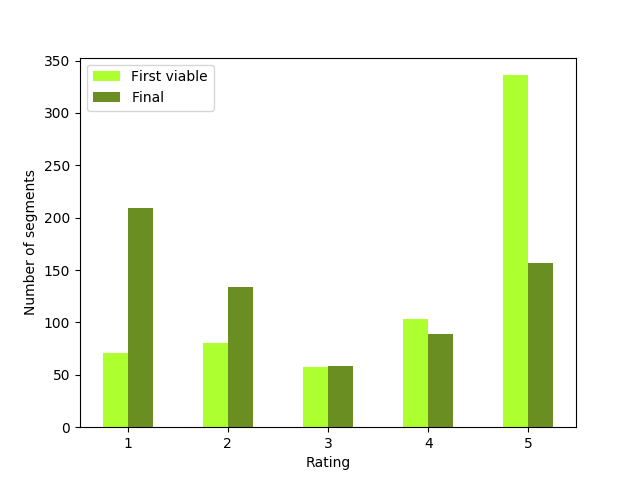
\includegraphics[width=0.8\linewidth]{img/experiment/qa_buckets.png}
    \caption{\label{fig:qa_buckets} Histogram of ratings for first viable and final translations (1 - best, 5 - worst)}
\end{figure}

The validation scores assigned to the individual segments using the histogram is presented in \cref{fig:qa_buckets}. We see that the first viable translations received mostly the worst rating while final hypotheses are bimodal: the majority received a favorable validation score but a considerable portion (24\%) had the worst score. We assume that in these cases, our setup was unreliable and fooled the user in accepting a misleading translation. A possible explanation of this is offered in \cref{sec:error_masking}.

Overall, this is a clear success, as our technique helps people to produce better messages in a language they do not speak. Nevertheless, it is important to mention the limitations of our pilot study. Our heuristics for picking first viable inputs may include sentences, which were actually not thought to be viable by the user. Maybe the sentences contained obvious errors, such as typos, which the user would fix anyway but maybe the user would not notice if we did not present the backtranslation. A more thorough exploration is needed to isolate such effects.

\subsubsection{Relation to sentence length}

One could expect that shorter sentences are generally easier to process by MT (except for very ambiguous very short sentences). To analyze this assumption in our setting, we plot the average validation score assigned to sentences based on the source length.

\begin{figure}[ht]
    \centering
    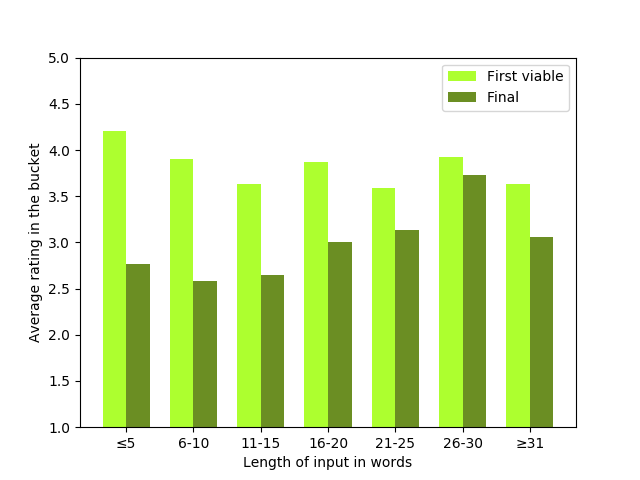
\includegraphics[width=0.8\linewidth]{img/experiment/qa_sentence_length.png}
    \caption{\label{fig:qa_sentence_length} Average rating for first viable and final translations based on the translated sentence length (1 - best, 5 - worst)}
\end{figure}

\cref{fig:qa_sentence_length} indicates that the assumed effect is not apparent in our case, at least not with our estimation of the first viable hypotheses. The shorter sentences generally receive worse validation scores than longer ones, but the differences are not very big.

For final hypotheses, the assumption seems more accurate: The best validation score was assigned to sentences of 6--10 words and the worst to sentences over 25 words. A noteworthy observation is that for these long sentences, the improvement in the validation scores from first viable to the final hypothesis is very low.

\subsection{Conclusion}

In this pilot experiment, users who did not know German were tasked to use this system for real-world use cases (communication with IT support, describing administrative issues and asking encyclopedic questions).

Across these domains, 5--10\,\% of inputs could not have been translated (our annotators have given up). For the submitted translations, the average self-reported confidence in the translations was 2.1 on a 1--5 (best--worst) scale and the tool was found more useful than standard web interfaces to MT (average usefulness of 1.71, same scale).

The majority of inputs were edited and while initial inputs and the final inputs were quite similar in the source language (word-level Gestalt Pattern Matching similarity of 75\,\%), the translations of them differed more (average similarity of 61\,\%).

The second, validation, phase of our experiment confirmed that the overall understandability of the translations improved from 3.9 to 2.71 on the 1--5 (best--worst) scale.

\pagebreak
\section{Changes in \ptakopet}
\label{sec:experiment_changes}

During the experiment, we acknowledged the need for separating experiment definitions from the rest of the code. As a result, the whole experiment content can be specified by a single JSON file instead of having to be hardcoded in the project. This is described in detail \cref{sec:experiment_def}. We also restructured the whole codebase, so that the experiment and settings profiles are more separated. The original version commit on which the pilot experiment took place got the \texttt{v-pilot} tag in the \texttt{zouharvi/ptakopet} repository.

In preparation for the next experiment we added a paraphrasing module visible in the bottom right corner in \cref{fig:experiment/stimuli_ui_new.png}

The experiment user interface also changed to accommodate better more modules and stimulus in the form of images. A stimuli is now confirmed by clicking one of the five buttons. They correspond to the confidence the user itself has of their produced texts (1 lowest -- 5 most). We added the ability to leave a note anywhere in the experiment by clicking the \text{NOTE} button below the rating scale. The progress is tracked visibly on the experiment page above the scale. This way, the annotators have a better overview of the amount of work left. All of the new features are shown in \cref{fig:experiment/stimuli_ui_new.png}.

\figcap{experiment/stimuli_ui_new.png}{Screenshot of the update \ptakopet{} interface for annotators with an image stimuli}

The baked stimuli queue is now split into blocks. They were added only for management purposes so that it is easier for users to split their work into several phases. They are notified by an alert box that they completed a block.

From the server point of view, nothing has been changed. Only the logs are now stored with \texttt{<userID>-<block>.log} scheme.